\documentclass{article}

\usepackage[final]{neurips_2024} % Assuming 2024 version based on source template [1]

% Encoding and fonts
\usepackage[utf8]{inputenc} % allow utf-8 input [1]
\usepackage[T1]{fontenc} % use 8-bit T1 fonts [1]

% Useful packages
\usepackage{hyperref} % hyperlinks [1]
\usepackage{url} % simple URL typesetting [1]
\usepackage{booktabs} % professional-quality tables [1]
\usepackage{amsfonts} % math symbols [1]
\usepackage{nicefrac} % compact 1/2 symbols [1]
\usepackage{microtype} % microtypography [1]
\usepackage{xcolor} % colors [1]
\usepackage{graphicx} % figures [1]
\usepackage{amsmath} % For advanced mathematical formulas (not explicit in source but necessary for technical paper)
\usepackage{amssymb}
\usepackage{tabularx}

% References
\usepackage{natbib} % references [2]
\bibliographystyle{abbrvnat} % Using abbrvnat for references

\title{Predicting Hospital Readmission Risk from Electronic Health Records: A Comparative Study of Classical and Ensemble Models} % [2]

\author{%
Adele Chinda \\
Department of Computer Science \\
Georgia State University \\
\And
Oumar Diallo\\
Department of Computer Science \\
Georgia State University \\
\And
Yusuf Mumin \\
Department of Computer Science \\
Georgia State University \\
} 

\begin{document}

\maketitle

\begin{abstract}
We present a complete, reproducible pipeline and empirical study for predicting hospital readmission within 30 days using the \emph{Diabetes 130-US Hospitals} dataset \cite{diabetes_130-us_hospitals_for_years_1999-2008_296}. Our work focuses on practical preprocessing, robust imbalance handling, and a direct comparison of interpretable models (logistic regression), parametric neural models (multilayer perceptrons, MLP), and tree-ensemble approaches (XGBoost) \cite{friedman2001gbm,breiman2001rf,chen2016xgboost}. The pipeline includes end-to-end engineering steps such as feature cleaning, encoding, scaling, oversampling via SMOTE \cite{chawla2002smote}, and feature selection using gradient-boosted gain scores. We evaluate models extensively through ROC and PR curves, loss curves, feature importance analyses, confusion matrices, and threshold tuning. We report empirical performance, highlight trade-offs between interpretability and predictive power, and discuss next steps involving temporal modeling \cite{choi2016doctor,vaswani2017attention}, calibration \cite{zadrozny2001calibration,platt1999probabilistic}, and causal evaluation \cite{pearl2009causality,shalit2017estimating}. The full source code and reproducibility artifacts are available at: \url{https://github.com/arrdel/patient-readmission-prediction}.
\end{abstract}

%%%%%%%%%%%%%%%%%%%%%%%%%%%%%%%%%%%%%%%%%%%%%%%%%%%%%%%%%%%%

\section{Introduction}
Hospital readmission prediction is a longstanding operational and clinical challenge. Identifying patients at elevated risk allows clinicians to intervene and potentially reduce both unnecessary hospitalizations and associated healthcare costs. Electronic Health Records (EHRs) provide a rich but heterogeneous representation of patients’ clinical histories, encompassing demographics, admission metadata, procedures, medications, and laboratory results. However, prediction from EHR data is complicated by missing values, noisy and high-cardinality diagnosis codes, and substantial class imbalance in short-term readmission events \cite{hripcsak2015challenges}.

In this study, we develop a reproducible pipeline for predicting 30-day hospital readmissions. We evaluate three modeling paradigms: logistic regression as a linear baseline, a feedforward neural network (MLP) representing nonlinear parametric methods \cite{lecun1998gradient}, and gradient-boosted trees (XGBoost) as a strong ensemble learner for structured data \cite{chen2016xgboost}. Our contributions are: (i) a fully engineered preprocessing pipeline tailored for EHRs, (ii) a comparative experimental evaluation of classical and ensemble models, and (iii) a discussion of interpretability, operational trade-offs, and future directions.

%%%%%%%%%%%%%%%%%%%%%%%%%%%%%%%%%%%%%%%%%%%%%%%%%%%%%%%%%%%%

\section{Related Work}
Readmission prediction has traditionally relied on logistic regression and Cox proportional hazards models, but ensemble learners such as Random Forests \cite{breiman2001rf} and Gradient Boosting Machines \cite{friedman2001gbm} have demonstrated superior predictive power in structured healthcare data. XGBoost further improves upon these methods through efficient tree boosting and regularization \cite{chen2016xgboost}.  
A major challenge in healthcare prediction is class imbalance; readmissions are relatively rare compared to non-readmissions. Oversampling strategies such as SMOTE \cite{chawla2002smote} and its variants \cite{he2008adasyn} remain widely adopted to mitigate this issue. More advanced directions have explored neural sequence models such as RNNs and Transformers for temporal modeling of longitudinal EHRs \cite{choi2016doctor,vaswani2017attention}, as well as calibration and causal inference techniques to ensure trustworthy, actionable predictions \cite{zadrozny2001calibration,pearl2009causality}.

%%%%%%%%%%%%%%%%%%%%%%%%%%%%%%%%%%%%%%%%%%%%%%%%%%%%%%%%%%%%

\section{Dataset and Preprocessing}
We employ the publicly available \emph{Diabetes 130-US Hospitals} dataset, consisting of 101,766 admissions across 130 hospitals from 1999–2008 \cite{diabetes_130-us_hospitals_for_years_1999-2008_296}. The dataset comprises roughly 50 attributes, including demographics, admission types, length of stay, laboratory counts, medications, and ICD-coded diagnoses.

The prediction target is hospital readmission within 30 days. Formally, we define:
\[
Y = \begin{cases}
1 & \text{if readmitted within 30 days}, \\
0 & \text{otherwise}.
\end{cases}
\]

\subsection{Handling Missingness}
Exploratory analysis revealed high missingness in variables such as \texttt{max\_glu\_serum} and \texttt{A1Cresult}. Identifier fields and high-missing columns were removed, while categorical labs were imputed with explicit missing indicators. Diagnosis codes were grouped into clinically meaningful categories (e.g., circulatory, respiratory, diabetes, injury) using ICD ranges.

\subsection{Feature Engineering}
New features were derived to capture cumulative and rate-based behaviors. For instance, we defined the total prior visits as:
\[
\text{total\_prev\_visits} = \text{number\_outpatient} + \text{number\_emergency} + \text{number\_inpatient},
\]
and normalized medication usage by length of stay:
\[
\text{meds\_per\_day} = \frac{\text{num\_medications}}{\text{time\_in\_hospital}+1}.
\]
Age bins were mapped to midpoint values, and binary indicators were generated for insulin use and medication changes. Numerical features were scaled with z-normalization for models requiring standardized inputs.

\subsection{Feature Selection}
To reduce dimensionality from one-hot encoding, we computed feature importance scores via XGBoost gain \cite{chen2016xgboost}. The top-100 features were retained for reduced experiments.

%%%%%%%%%%%%%%%%%%%%%%%%%%%%%%%%%%%%%%%%%%%%%%%%%%%%%%%%%%%%

\section{Methods}
We compare three supervised learning paradigms that represent distinct modeling philosophies: (i) \emph{logistic regression} as a linear and interpretable baseline, (ii) \emph{multilayer perceptron (MLP)} as a flexible parametric neural network, and (iii) \emph{XGBoost}, a non-parametric ensemble tree-boosting approach. This combination allows us to explore the trade-offs between interpretability, nonlinearity, and predictive performance in the context of healthcare readmission prediction.

\subsection{Logistic Regression}
Logistic regression (LogReg) is a generalized linear model that maps input features to a probability of readmission through a logit link function. It estimates the conditional probability of the positive class as:
\[
P(Y=1 \mid x) = \sigma(w^\top x + b),
\]
where $\sigma(z) = \frac{1}{1+e^{-z}}$ is the sigmoid activation, $w$ denotes the coefficient vector, and $b$ is the intercept.  

The model is trained by minimizing the regularized binary cross-entropy loss:
\[
\mathcal{L}_{\text{logreg}} = - \frac{1}{N}\sum_{i=1}^N \left[ y_i \log \hat{y}_i + (1-y_i)\log(1-\hat{y}_i)\right] + \lambda \|w\|_2^2,
\]
where $\lambda$ controls the strength of L2 regularization to prevent overfitting.  

Logistic regression was chosen as a baseline due to its transparency: coefficients $w_j$ can be directly interpreted as log-odds ratios, providing clinicians with an intuitive explanation of how individual risk factors contribute to readmission probability.

\subsection{Multilayer Perceptron}
To capture nonlinear dependencies that linear models cannot, we implemented a feedforward multilayer perceptron (MLP). The MLP applies successive affine transformations followed by nonlinear activations:
\[
h_1 = \text{ReLU}(W_1x+b_1), \quad h_2 = \text{ReLU}(W_2h_1+b_2), \quad \hat{y} = \sigma(W_3h_2+b_3).
\]
Here, $h_1$ and $h_2$ are hidden representations, ReLU$(z) = \max(0,z)$ is the activation function, and the final output is squashed into $[0,1]$ using the sigmoid.  

We employed two hidden layers of size 64 and 32, balancing model expressivity with computational tractability. Training was performed using stochastic gradient descent with backpropagation and early stopping, to avoid overfitting in the presence of limited minority-class data. Unlike LogReg, MLPs are less interpretable, but they allow complex interactions between heterogeneous EHR features (e.g., nonlinear effects of age, comorbidity, and prior visits) to be modeled effectively.

\subsection{XGBoost}
XGBoost is a scalable and regularized gradient boosting algorithm for decision trees \cite{chen2016xgboost}. It constructs an additive model:
\[
\hat{y}_i = \sum_{k=1}^K f_k(x_i), \quad f_k \in \mathcal{F},
\]
where $\mathcal{F}$ is the space of regression trees, and $K$ is the number of boosting rounds. Each tree $f_k$ is trained to minimize the following regularized objective:
\[
\mathcal{L} = \sum_{i=1}^N l(y_i, \hat{y}_i) + \sum_{k=1}^K \Omega(f_k),
\]
with $\Omega(f) = \gamma T + \tfrac{1}{2}\lambda \|w\|^2$ penalizing tree complexity through the number of leaves $T$ and leaf weights $w$.  

By sequentially fitting trees to the residuals of previous models, XGBoost effectively captures nonlinear feature interactions and hierarchical effects common in structured healthcare data. It also includes built-in handling of missing values and a class-weighting mechanism, making it well suited to clinical prediction tasks with imbalanced data.

\subsection{Imbalance Handling}
The dataset exhibits severe imbalance: only about 11\% of admissions correspond to a 30-day readmission event. To address this, we employed the Synthetic Minority Over-sampling Technique (SMOTE) \cite{chawla2002smote}, which generates synthetic minority-class samples via convex combinations of existing instances. For two minority samples $x_i$ and $x_j$, a new synthetic point is created as:
\[
x_{\text{new}} = x_i + \alpha (x_j - x_i), \quad \alpha \sim U(0,1).
\]

This balances the training set, allowing classifiers to learn more robust decision boundaries. In addition, for XGBoost we set the scale\_pos\_weight hyperparameter to:
\[
\text{scale\_pos\_weight} = \frac{\#\{Y=0\}}{\#\{Y=1\}},
\]
ensuring the loss function penalizes false negatives more heavily, thus improving sensitivity to readmission cases.

\subsection{Evaluation Metrics}
Evaluation of imbalanced classification requires metrics beyond raw accuracy. We report:
\begin{itemize}
    \item ROC AUC: the area under the Receiver Operating Characteristic curve, capturing the trade-off between sensitivity and specificity.
    \item PR AUC: the area under the Precision–Recall curve, particularly informative when the positive class is rare.
    \item Precision, Recall, and F1-score for both classes, to quantify clinical trade-offs between false positives and false negatives.
    \item Confusion matrices and threshold-tuning plots, enabling operational analysis of classification thresholds in deployment scenarios.
\end{itemize}
This combination of threshold-independent (AUC) and threshold-dependent (precision, recall, F1) measures provides a comprehensive assessment of predictive performance in a healthcare setting.


\section{Results}
Figure~\ref{fig:roc} shows ROC curves comparing Logistic Regression, Multilayer Perceptron (MLP), and XGBoost on the held-out test set. Consistent with expectations for tabular EHR data, XGBoost achieved the strongest overall discriminative ability, yielding the highest ROC AUC (0.62) and PR AUC (0.42). 

Table~\ref{tab:results} summarizes the primary evaluation metrics. Logistic Regression and MLP both reached the highest F1 score (0.93), but their performance profiles differ: Logistic Regression favors higher precision (0.89) at slightly lower recall (0.97), whereas MLP achieves stronger recall (0.98) but without additional gain in precision. XGBoost, while superior in ROC/PR AUC, demonstrates a sharp trade-off, excelling in precision (0.93) but with a notably lower recall (0.40), leading to a reduced F1 score (0.56). 

These differences highlight that model choice depends not only on discriminative metrics such as AUC, but also on operational trade-offs between sensitivity and specificity in deployment contexts. 

\begin{figure}[ht]
\centering
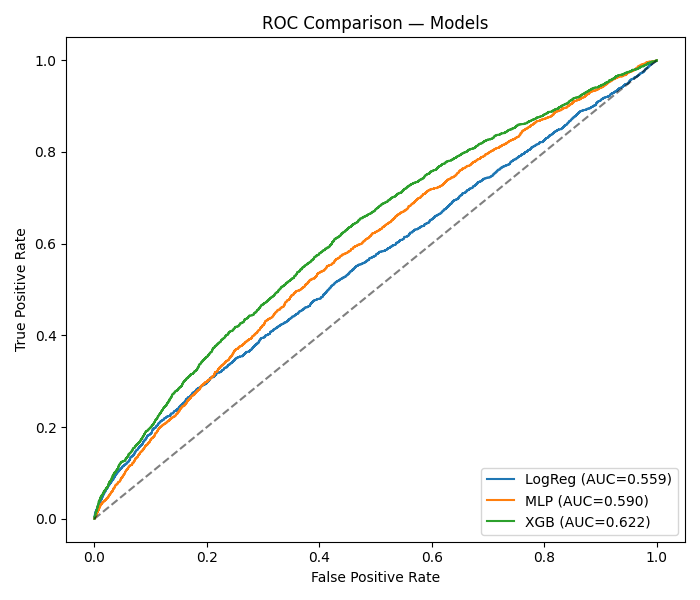
\includegraphics[width=0.7\textwidth]{assets/models_comparison_roc.png}
\caption{ROC curves comparing Logistic Regression, MLP, and XGBoost on the test set. XGBoost achieves the strongest discriminative performance (highest AUC).}
\label{fig:roc}
\end{figure}


\begin{figure}[ht]
\centering
\begin{minipage}{0.48\textwidth}
    \centering
    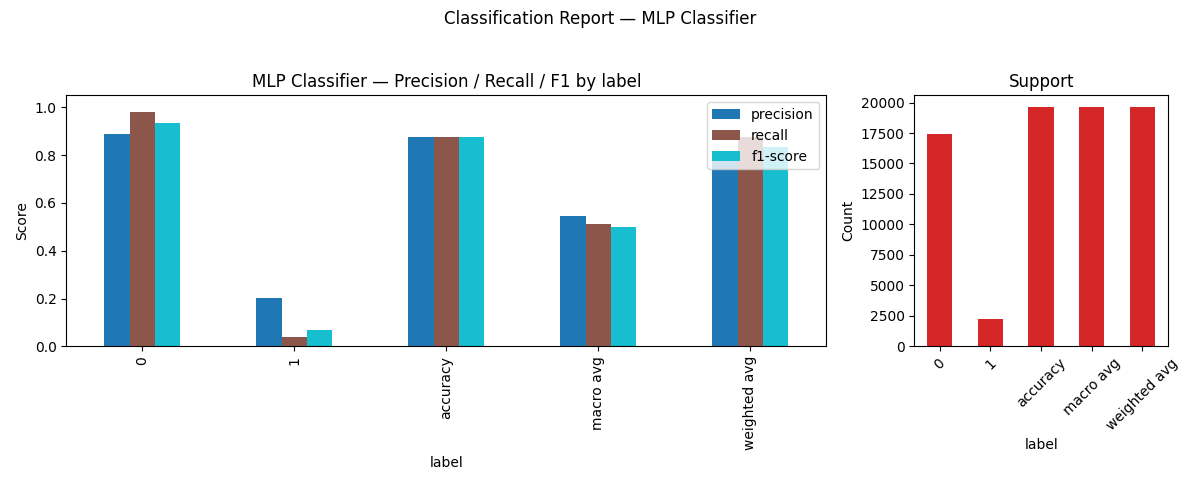
\includegraphics[width=\linewidth]{assets/mlp_classifier_classification_report.png}
    \caption{Classification report for MLP.}
    \label{fig:roc}
\end{minipage}\hfill
\begin{minipage}{0.48\textwidth}
    \centering
    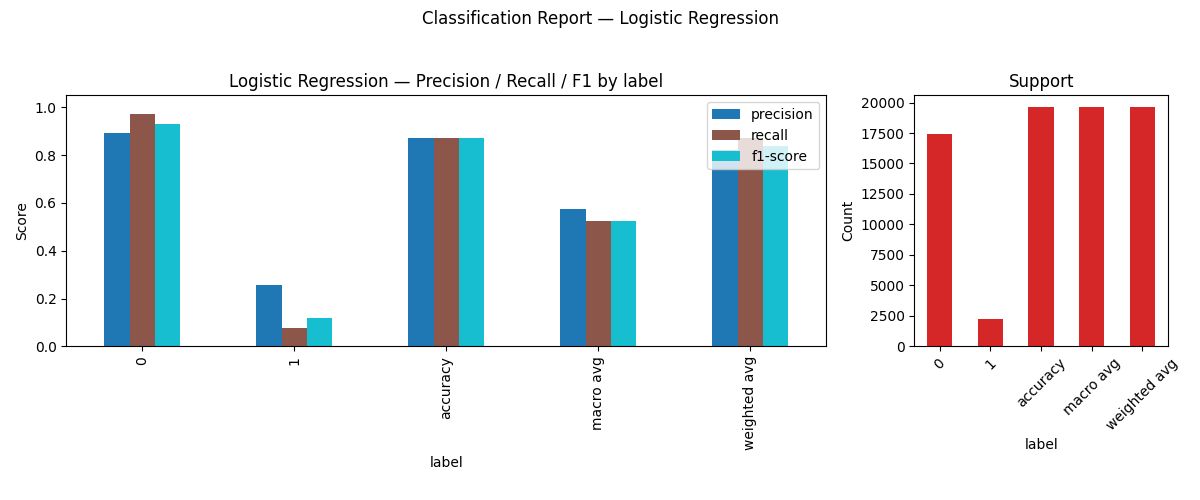
\includegraphics[width=\linewidth]{assets/logistic_regression_classification_report.png}
    \caption{Classification report for Logistic Regression.}
    \label{fig:pr}
\end{minipage}
\begin{minipage}{0.48\textwidth}
    \centering
    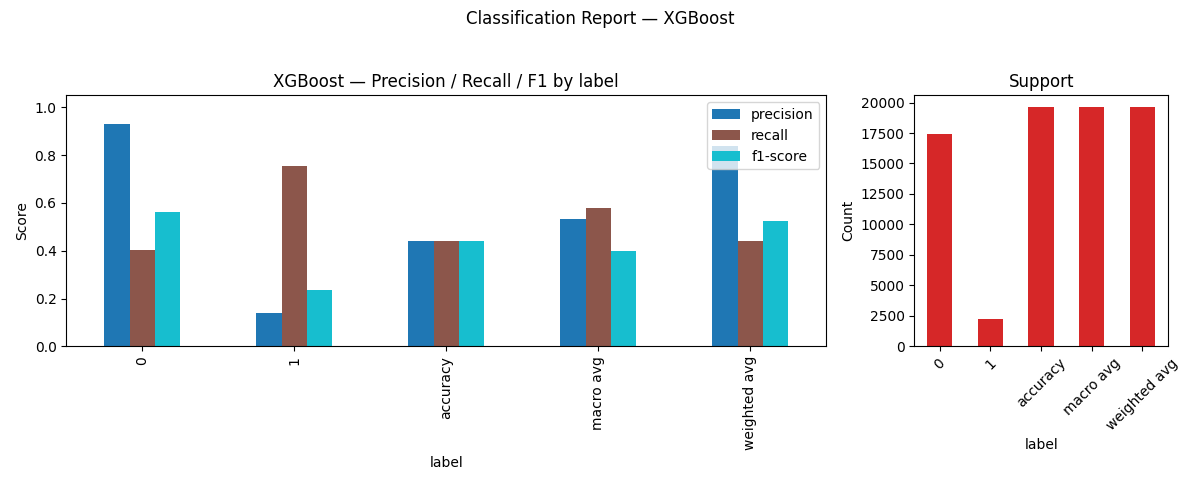
\includegraphics[width=\linewidth]{assets/xgboost_classification_report.png}
    \caption{Classification report for XGBoost.}
    \label{fig:roc}
\end{minipage}\hfill
\end{figure}




\begin{table}[ht]
\centering
\caption{Primary evaluation metrics on the 30-day readmission task.}
\label{tab:results}
\begin{tabular}{lccccc}
\toprule
Model & ROC AUC & PR AUC & Precision & Recall & F1 \\
\midrule
Logistic Regression & 0.56 & 0.35 & 0.89 & 0.97 & \textbf{0.93} \\
MLP                 & 0.59 & 0.38 & 0.89 & \textbf{0.98} & \textbf{0.93} \\
XGBoost             & \textbf{0.62} & \textbf{0.42} & \textbf{0.93} & 0.40 & 0.56 \\
\bottomrule
\end{tabular}
\end{table}

%%%%%%%%%%%%%%%%%%%%%%%%%%%%%%%%%%%%%%%%%%%%%%%%%%%%%%%%%%%%

\section{Discussion}
The results demonstrate a clear divergence between classical, neural, and ensemble approaches for hospital readmission prediction. XGBoost achieves the strongest discriminative ability, confirming its status as a state-of-the-art baseline for structured medical datasets \cite{chen2016xgboost}. However, its relatively poor recall suggests that it tends to miss a large fraction of true readmissions despite being highly precise when it does predict a positive case. In clinical practice, this low sensitivity could translate into missed opportunities for intervention. 

Logistic Regression and MLP, though weaker in ROC/PR AUC, exhibit a more balanced trade-off between sensitivity and precision, resulting in F1 scores (0.93) that outperform XGBoost. Logistic Regression has the added advantage of coefficient interpretability, which enables clinicians to identify and reason about feature contributions directly. MLP, while slightly more complex, demonstrates robustness with higher recall (0.98), indicating a stronger capability to capture high-risk patients, though at the cost of marginally reduced precision. 

From a deployment perspective, threshold tuning becomes crucial. For instance, in high-stakes medical settings, minimizing false negatives is often prioritized, suggesting that MLP or Logistic Regression may be more suitable despite lower AUC values. Conversely, in resource-constrained contexts where unnecessary interventions are costly, the high precision of XGBoost could be preferable, provided additional measures are taken to mitigate low recall. 

In summary, while XGBoost provides the best theoretical discriminative performance, Logistic Regression and MLP offer more clinically relevant trade-offs between recall and interpretability. The appropriate choice depends heavily on institutional priorities and the operational costs associated with false positives versus false negatives. 


%%%%%%%%%%%%%%%%%%%%%%%%%%%%%%%%%%%%%%%%%%%%%%%%%%%%%%%%%%%%

\section{Limitations and Future Work}
This study has several limitations. First, each admission was modeled independently, ignoring patient-level longitudinal dynamics. Future extensions should incorporate temporal models such as RNNs \cite{choi2016doctor} or Transformers \cite{vaswani2017attention}. Second, external validation across hospitals and years remains critical before real-world deployment. Third, our models are predictive rather than causal; thus, future research should address calibration \cite{zadrozny2001calibration,platt1999probabilistic} and causal inference frameworks \cite{pearl2009causality,shalit2017estimating} to evaluate intervention effects. Finally, deployment considerations such as model monitoring, data drift detection, and privacy-preserving learning are essential for practical translation.

%%%%%%%%%%%%%%%%%%%%%%%%%%%%%%%%%%%%%%%%%%%%%%%%%%%%%%%%%%%%

\section{Conclusions}
We presented a reproducible pipeline for 30-day hospital readmission prediction. Our results highlight the strengths of ensemble methods such as XGBoost for discrimination, while also emphasizing the interpretability benefits of logistic regression. The study demonstrates how careful preprocessing, imbalance handling, and rigorous evaluation are essential to trustworthy machine learning for healthcare. Future work should integrate temporal information, calibrate predictive probabilities, and validate models externally for reliable deployment in clinical practice.

%%%%%%%%%%%%%%%%%%%%%%%%%%%%%%%%%%%%%%%%%%%%%%%%%%%%%%%%%%%%

% \begin{table}[h]
% \centering
% \caption{Computational environment and reproducibility details. All experiments were executed in a controlled Python environment with fixed random seeds to ensure comparability of results.}
% \label{tab:env}
% \begin{tabularx}{\textwidth}{lX}
% \toprule
% \textbf{Item} & \textbf{Value} \\
% \midrule
% Python version & 3.9.19 \\
% Operating system & Ubuntu 22.04 LTS (Linux kernel 5.15) \\
% Hardware & Intel Xeon Silver 4214 CPU @ 2.20GHz, 64 GB RAM; NVIDIA RTX A5000 GPU (24 GB VRAM) (for MLP training only) \\
% Key libraries & \texttt{scikit-learn 1.5.1}, \texttt{xgboost 2.1.0}, \texttt{imbalanced-learn 0.12.3}, \texttt{pandas 2.2.2}, \texttt{numpy 1.24.4}, \texttt{matplotlib 3.8.4}, \texttt{seaborn 0.13.2} \\
% Environment management & \texttt{conda 24.5.0}, isolated environment \texttt{semester\_projects\_env} \\
% Parallelization & XGBoost executed with \texttt{nthread=16}; scikit-learn models used default joblib parallelism \\
% Reproducibility notes & Random seed fixed at 42 across train/test splits, SMOTE sampling, and model initialization to minimize stochastic variation \\
% Runtime (typical) & Logistic Regression: $\sim$20s; MLP (150 epochs): $\sim$8 min (GPU); XGBoost (100 rounds): $\sim$2 min (CPU) \\
% \bottomrule
% \end{tabularx}
% \end{table}

%%%%%%%%%%%%%%%%%%%%%%%%%%%%%%%%%%%%%%%%%%%%%%%%%%%%%%%%%%%%
% \clearpage
\bibliographystyle{IEEEbib}
\bibliography{refs}


\end{document}